
\section{\ref{PS:Q:Performance}}

\textit{Can we create a solution that scales such that the number of turbines does not impact the regulation cycle time?}

\subsection{Experimenit}
\label{sec:Exper:perfom}

%Scalability is by Bondi\cite{Bondi:2000:CSI:350391.350432} defined as \textit{the systems ability to accommodate an increasing number of elements or objects, to process growing volumes of work gracefully, and/or to be susceptible to enlargement}.

The \ref{PS:Q:Performance} question asks if the proposed decentralized system is able to scale with the number of turbines in the system. The experiments that investigate this question has been split into two part. \newline

Part 1 aims to investigate the anticorrelation between regulation time and cache read count in the proposed decentralized system. This is relevant because changing the regulation time may have an impact on the number of cache reads. Choosing a regulation time that has a low number of cache read count for part 2 of the experiments will make it easier to identify how scaling up the number of turbines will affect cache read count. \newline

Part 2 aims to investigate the impact on regulation time and cache read count when the number of turbines are scaled up in the proposed decentralized system. \newline

\subsection{Part 1: Regulation time and the impact on cache read count}
\label{subsec:Exper:perfom:1}
The experiment below are made to show how the regulation time affect the cache read count in the decentralized system described in \cref{cha:decentralizedSystem}. 
The experiments are performed with \testCycletimeNumbers ~cycle times.  

The following procedure is used each time the experiment is performed:
\begin{enumerate}
	\item Start the system with a cycle time of N ms and 21 turbines.
	\item Make sure the system is stable.
	\item Start logging the reported regulation run time and cache read count.
	\item Stop logging after \experiemntRunTime.
\end{enumerate}

\subsection{Part 2: Number of turbines and their impact on regulation time and cache read count}
\label{subsec:Exper:perfom:2}
The experiment below are made to show how the number of turbines affect the regulation cycle in the decentralized system described in \cref{cha:decentralizedSystem}.

The experiments are performed with \testTurbineNumbers ~turbines. Besides turbines we are also going to modify ''Data Wait Time Frame'' witch is a constant that defines the time a turbine controller will wait for new updates before considering the other turbines offline and unavailable, i.e. regulation speed.

The test system is expected to be running only one instance in a real life implementation, therefore the test machine will only run one instance and the support machines will run the rest generating system load.
The experiment is done with a variating N number of online turbines.

The following procedure is used each time the experiment is performed:
\begin{enumerate}
	\item Start the system with N turbines.
	\item Make sure the system is stable.
	\item Start logging the reported regulation run time and cache read count.
	\item Stop logging after \experiemntRunTime.
\end{enumerate}


\subsection{Results}

\label{sec:exp:performance}
The cycle times are calculated as the difference between the receive timestamp of the oldest turbine state package and a timestamp right after the new turbine state has been sent and the turbines setpoint has been set.
The regulation cycle time with variating number of turbines are done with box plots and a line. The box plots whiskers show the extreme values max and min, the top and bottom of the box show the upper and lower quartile of the data, and the center line shows the median. The median is further highlighted by a line.

\subsubsection{\nameref{subsec:Exper:perfom:1}}

The results of one of the \nameref{sec:Exper:perfom} experiments plotted are plotted in \cref{fig:exp:decen:sleep,fig:exp:decen:sleep-cache}.
The experiment where performed with a variating number of internal wait times.

\begin{figure}[h!]
	\centering
	\begin{tikzpicture}
\begin{axis}
[
width=\resultsFigureWidthScale\textwidth,
axis y line*=left,
xlabel=Sleeptime (ms),
ylabel=Regulation cycle time (ms),
ymin = 0,
xtick={1, 2, 3, 4, 5, 6, 7, 8, 9},
xticklabels={10, 15, 20, 25, 30, 35, 40, 45, 50},
boxplot/draw direction=y
]

%% /home/stefan/work/TestResults/Test6_Decentralized_12-7-2014_1327/nCycleTime/DecentralizedLog1.csv
\buildBoxPlot{10.578002}{15.286001}{9.942}{148.911}{0.415002}

%% /home/stefan/work/TestResults/Test6_Decentralized_12-7-2014_1327/nCycleTime/DecentralizedLog2.csv
\buildBoxPlot{15.026002}{15.383002}{14.312002}{26.729001}{1.379}

%% /home/stefan/work/TestResults/Test6_Decentralized_12-7-2014_1327/nCycleTime/DecentralizedLog3.csv
\buildBoxPlot{19.926}{20.380001}{18.979001}{29.932002}{0.435}

%% /home/stefan/work/TestResults/Test6_Decentralized_12-7-2014_1327/nCycleTime/DecentralizedLog4.csv
\buildBoxPlot{25.079001}{25.322}{24.637001}{32.794001}{12.225002}

%% /home/stefan/work/TestResults/Test6_Decentralized_12-7-2014_1327/nCycleTime/DecentralizedLog5.csv
\buildBoxPlot{30.099}{30.363}{29.565001}{42.436}{4.466}

%% /home/stefan/work/TestResults/Test6_Decentralized_12-7-2014_1327/nCycleTime/DecentralizedLog6.csv
\buildBoxPlot{35.153001}{35.328002}{34.853001}{45.836001}{10.347}

%% /home/stefan/work/TestResults/Test6_Decentralized_12-7-2014_1327/nCycleTime/DecentralizedLog7.csv
\buildBoxPlot{40.157001}{40.434001}{39.626}{58.338001}{6.398001}

%% /home/stefan/work/TestResults/Test6_Decentralized_12-7-2014_1327/nCycleTime/DecentralizedLog8.csv
\buildBoxPlot{45.185}{45.330001}{44.928002}{50.089}{29.313}

%% /home/stefan/work/TestResults/Test6_Decentralized_12-7-2014_1327/nCycleTime/DecentralizedLog9.csv
\buildBoxPlot{49.958002}{50.391001}{49.019}{64.611002}{4.846}


\addplot[thick, red!70] coordinates {
	(1 ,10.578002)
	(2 ,15.026002)
	(3 ,19.926)
	(4 ,25.079001)
	(5 ,30.099)
	(6 ,35.153001)
	(7 ,40.157001)
	(8 ,45.185)
	(9 ,49.958002)
	
};

\end{axis}
\end{tikzpicture}

	\caption{Decentralized solution with variable wait time cycle time experiment}
	\label{fig:exp:decen:sleep}
\end{figure}

\Cref{fig:exp:decen:sleep} show the that the regulation cycle times and wait times are linearly Dependant on each other, the maximum value with wait time 10 is outside the boundaries of the plot but is calculated to 148.91 ms The upper and lower quartile are close together the exception is the 10 ms wait time sample, the maximum being the 20 ms wait time having a difference of 1.401 ms between upper and lower quantile and the minimum being 45 ms wait time with a difference of 0.402 ms The maximum values again with the exception of the 10 ms wait time sample follow the median values, the minimum values are able to reach low regulation cycle times much lower than the wait time used in the experiment.

\begin{figure}[h!]
	\centering
	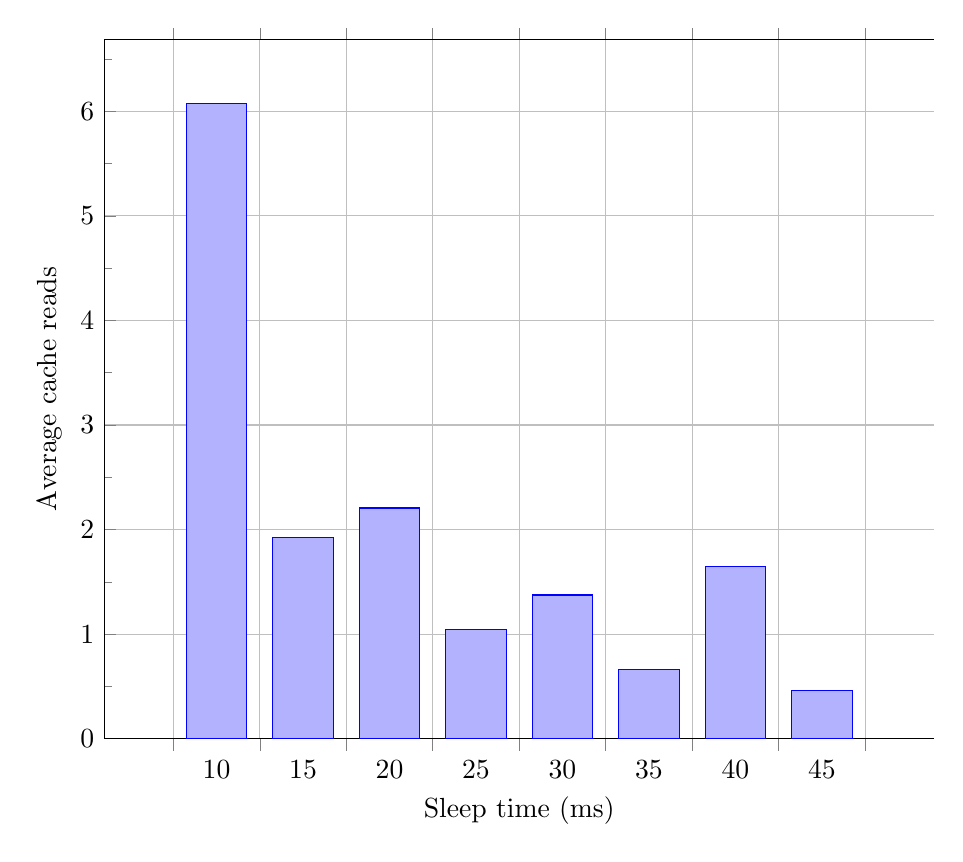
\begin{tikzpicture}
\begin{axis}
[
width=\resultsPlotWidthScale\textwidth,
axis y line*=left,
xlabel=Sleep time (ms),
ymin = 0,
%xmin = 0,
ylabel=Average cache reads,
%xtick={1, 2, 3, 4, 5, 6, 7, 8, 9},
%xticklabels={10, 15, 20, 25, 30, 35, 40, 45, 50},
%boxplot/draw direction=y,
%grid=both,
%ymajorgrids=true,
%yminorgrids=true,
ybar interval=0.7,
ymajorgrids=true,
%yminorgrids=true,
minor y tick num=1
%minor tick num=1
]
%\buildBoxPlot[black]{0}{0}{0}{0}{0}
%\buildBoxPlot[black]{0}{0}{0}{0}{0}
%\buildBoxPlot[black]{0}{0}{0}{0}{0}
%\buildBoxPlot[black]{0}{0}{0}{0}{0}
%\buildBoxPlot[black]{0}{0}{0}{0}{0}
%\buildBoxPlot[black]{0}{0}{0}{0}{0}
%\buildBoxPlot[black]{0}{0}{0}{0}{0}
%\buildBoxPlot[black]{0}{0}{0}{0}{0}
%\buildBoxPlot[black]{0}{0}{0}{0}{0}
\addplot coordinates {
	(10 ,6.076278918444858)
	(15 ,1.9250837336102817)
	(20 ,2.206446850393701)
	(25 ,1.044688862465319)
	(30 ,1.3747593094220163)
	(35 ,0.661782154722354)
	(40 ,1.6464805561590268)
	(45 ,0.46317152740208856)
	(50 ,1.858914282814271)
};

%matlab info
%     General model:
%     f(x) = (a/(x+b))+ c
%     Coefficients (with 95% confidence bounds):
%     a =       7.017  (-8.781, 22.82)
%     b =      -8.622  (-11.55, -5.697)
%     c =      0.9821  (0.01249, 1.952)
     
%\addplot[
%red,
%domain=10:50,
%samples=201,
%]
%{(7.017/(x-8.622))+ 0.9821};

\end{axis}
\end{tikzpicture}
	\caption{Decentralized solution with variable wait time cache reads experiment}
	\label{fig:exp:decen:sleep-cache}
\end{figure}

\Cref{fig:exp:decen:sleep-cache} show the average cache reads of the experiment.
A cache read only happens in the decentralized solution and is a consequence of the separation of receiving data in a separate thread.
The cache read happens if the wait time elapses before all turbine instances have responded with state information. The Number dos not include information of if the same turbine instance state has been read from cache multiple times.
The number of cache reads is declining. 
%, a fitted function of the plot has been put on top (red), the plot is in Matlab fitted against the function $\dfrac{a}{x + b} + c$.

\clearpage
\subsubsection{\nameref{subsec:Exper:perfom:2}}
The plots in this section relates to the second part of the \nameref{sec:Exper:perfom} experiment. In this graph the regulation cycle time is plotted against a variating number of turbines.

\begin{figure}[h!]
	\centering
	\begin{tikzpicture}
\begin{axis}
[
width=\textwidth,
axis y line*=left,
xlabel=Number of turbines,
ylabel=Regulation cycle time (ms),
ymin = 0,
xtick={1, 2, 3, 4, 5, 6, 7, 8, 9, 10, 11, 12, 13, 14, 15, 16, 17, 18, 19, 20},
xticklabels={5, 10, 15, 20, 25, 30, 35, 40, 45, 50, 55, 60, 65, 70, 75, 80, 85, 90, 95, 100},
boxplot/draw direction=y
]

%% /home/stefan/work/TestResults/Test5_Decentralized_success_12-4-2014_2100/nTurbines/DecentralizedLog0.csv
\buildBoxPlot{19.526002}{20.412002}{15.272001}{26.620001}{0.282}

%% /home/stefan/work/TestResults/Test5_Decentralized_success_12-4-2014_2100/nTurbines/DecentralizedLog1.csv
\buildBoxPlot{20.257002}{20.365001}{20.158001}{24.403002}{0.828002}

%% /home/stefan/work/TestResults/Test5_Decentralized_success_12-4-2014_2100/nTurbines/DecentralizedLog2.csv
\buildBoxPlot{20.221001}{20.311002}{20.126002}{24.641001}{3.778}

%% /home/stefan/work/TestResults/Test5_Decentralized_success_12-4-2014_2100/nTurbines/DecentralizedLog3.csv
\buildBoxPlot{20.203002}{20.321002}{20.066}{24.962}{0.246002}

%% /home/stefan/work/TestResults/Test5_Decentralized_success_12-4-2014_2100/nTurbines/DecentralizedLog4.csv
\buildBoxPlot{20.174001}{20.343}{19.946}{25.983002}{0.273002}

%% /home/stefan/work/TestResults/Test5_Decentralized_success_12-4-2014_2100/nTurbines/DecentralizedLog5.csv
\buildBoxPlot{20.190001}{20.286002}{20.051}{24.771001}{10.959001}

%% /home/stefan/work/TestResults/Test5_Decentralized_success_12-4-2014_2100/nTurbines/DecentralizedLog6.csv
\buildBoxPlot{20.079}{20.391001}{19.563001}{27.503001}{0.371002}

%% /home/stefan/work/TestResults/Test5_Decentralized_success_12-4-2014_2100/nTurbines/DecentralizedLog7.csv
\buildBoxPlot{20.176}{20.303001}{19.965}{30.63}{9.225}

%% /home/stefan/work/TestResults/Test5_Decentralized_success_12-4-2014_2100/nTurbines/DecentralizedLog8.csv
\buildBoxPlot{19.998}{20.351001}{19.215}{30.385002}{0.543001}

%% /home/stefan/work/TestResults/Test5_Decentralized_success_12-4-2014_2100/nTurbines/DecentralizedLog9.csv
\buildBoxPlot{20.008}{20.384001}{19.068001}{29.380001}{4.096002}

%% /home/stefan/work/TestResults/Test5_Decentralized_success_12-4-2014_2100/nTurbines/DecentralizedLog10.csv
\buildBoxPlot{19.902002}{20.353}{18.909001}{33.447001}{2.831002}

%% /home/stefan/work/TestResults/Test5_Decentralized_success_12-4-2014_2100/nTurbines/DecentralizedLog11.csv
\buildBoxPlot{19.937001}{20.373}{18.991001}{33.877001}{1.672002}

%% /home/stefan/work/TestResults/Test5_Decentralized_success_12-4-2014_2100/nTurbines/DecentralizedLog12.csv
\buildBoxPlot{20.056}{20.415001}{19.421002}{40.952001}{0.923001}

%% /home/stefan/work/TestResults/Test5_Decentralized_success_12-4-2014_2100/nTurbines/DecentralizedLog13.csv
\buildBoxPlot{20.215}{21.471}{19.378}{151.296001}{0.528001}

%% /home/stefan/work/TestResults/Test5_Decentralized_success_12-4-2014_2100/nTurbines/DecentralizedLog14.csv
\buildBoxPlot{19.920001}{20.535002}{18.897001}{53.699}{0.768}

%% /home/stefan/work/TestResults/Test5_Decentralized_success_12-4-2014_2100/nTurbines/DecentralizedLog15.csv
\buildBoxPlot{20.129002}{21.354002}{18.846002}{69.145001}{0.589001}

%% /home/stefan/work/TestResults/Test5_Decentralized_success_12-4-2014_2100/nTurbines/DecentralizedLog16.csv
\buildBoxPlot{20.189001}{22.247}{18.578001}{89.297001}{0.707}

%% /home/stefan/work/TestResults/Test5_Decentralized_success_12-4-2014_2100/nTurbines/DecentralizedLog17.csv
\buildBoxPlot{20.902001}{25.559001}{18.828}{142.836}{0.615001}

%% /home/stefan/work/TestResults/Test5_Decentralized_success_12-4-2014_2100/nTurbines/DecentralizedLog18.csv
\buildBoxPlot{25.609001}{35.368002}{20.078002}{150.034001}{0.579001}

%% /home/stefan/work/TestResults/Test5_Decentralized_success_12-4-2014_2100/nTurbines/DecentralizedLog19.csv
\buildBoxPlot{36.934001}{53.153001}{24.836001}{150.673002}{0.684001}


\addplot[thick, red!70] coordinates {
	(1 ,19.526002)
	(2 ,20.257002)
	(3 ,20.221001)
	(4 ,20.203002)
	(5 ,20.174001)
	(6 ,20.190001)
	(7 ,20.079)
	(8 ,20.176)
	(9 ,19.998)
	(10 ,20.008)
	(11 ,19.902002)
	(12 ,19.937001)
	(13 ,20.056)
	(14 ,20.215)
	(15 ,19.920001)
	(16 ,20.129002)
	(17 ,20.189001)
	(18 ,20.902001)
	(19 ,25.609001)
	(20 ,36.934001)
	
};

\end{axis}
\end{tikzpicture}
\begin{tikzpicture}
\begin{axis}
[
width=\textwidth,
axis y line*=left,
xlabel=Number of turbines,
ymin = 0,
ylabel=Average Cache hits,
xtick={1, 2, 3, 4, 5, 6, 7, 8, 9, 10, 11, 12, 13, 14, 15, 16, 17, 18, 19, 20},
xticklabels={5, 10, 15, 20, 25, 30, 35, 40, 45, 50, 55, 60, 65, 70, 75, 80, 85, 90, 95, 100},
boxplot/draw direction=y
]
\buildBoxPlot[black]{0}{0}{0}{0}{0}
\buildBoxPlot[black]{0}{0}{0}{0}{0}
\buildBoxPlot[black]{0}{0}{0}{0}{0}
\buildBoxPlot[black]{0}{0}{0}{0}{0}
\buildBoxPlot[black]{0}{0}{0}{0}{0}
\buildBoxPlot[black]{0}{0}{0}{0}{0}
\buildBoxPlot[black]{0}{0}{0}{0}{0}
\buildBoxPlot[black]{0}{0}{0}{0}{0}
\buildBoxPlot[black]{0}{0}{0}{0}{0}
\buildBoxPlot[black]{0}{0}{0}{0}{0}
\buildBoxPlot[black]{0}{0}{0}{0}{0}
\buildBoxPlot[black]{0}{0}{0}{0}{0}
\buildBoxPlot[black]{0}{0}{0}{0}{0}
\buildBoxPlot[black]{0}{0}{0}{0}{0}
\buildBoxPlot[black]{0}{0}{0}{0}{0}
\buildBoxPlot[black]{0}{0}{0}{0}{0}
\buildBoxPlot[black]{0}{0}{0}{0}{0}
\buildBoxPlot[black]{0}{0}{0}{0}{0}
\buildBoxPlot[black]{0}{0}{0}{0}{0}
\buildBoxPlot[black]{0}{0}{0}{0}{0}
\addplot[thick, orange!70] coordinates {
	(1 ,0.2591015249347438)
	(2 ,0.3423283799799435)
	(3 ,0.4286200856364344)
	(4 ,0.7913519050319182)
	(5 ,1.171919068056407)
	(6 ,0.4440826120490188)
	(7 ,1.8595523144717856)
	(8 ,0.506366007056297)
	(9 ,1.8951768000539848)
	(10 ,2.037951753081981)
	(11 ,2.0728170589196186)
	(12 ,2.0275369832294468)
	(13 ,1.2416290071090674)
	(14 ,3.5220372523313626)
	(15 ,2.115832267020478)
	(16 ,3.7417427229878832)
	(17 ,5.311682134712245)
	(18 ,8.473847137142263)
	(19 ,14.663734246038112)
	(20 ,22.06932793366117)
};
\end{axis}
\end{tikzpicture}
	\caption{Decentralized solution variable number of turbines experiment 1}
	\label{fig:exp:decen:turbines}
\end{figure}

\cref{fig:exp:decen:turbines} show regulation cycle time of the decentralized system compared with a variating number of turbines. The internal sleep parameter is fixed as 20~ms
It is seen the system performs with a constant regulation cycle time with 5 to 90 turbines, if only observing the median.
The quartiles are with the exception of the 5 turbines experiment of almost constant until 65, the same applies to the maximum values.
The extreme regulation cycle time values all  stop close to 150 ms.
At 70 turbines the maximum value sticks out notably it does look like a outlier however checking the raw data, it is not there are logged regulation cycle times for every ms value between it and the median.
It should be noted that all the data with a cycle time above 132~ms are collected from the same test machine.

\begin{figure}[h!]
	\centering
	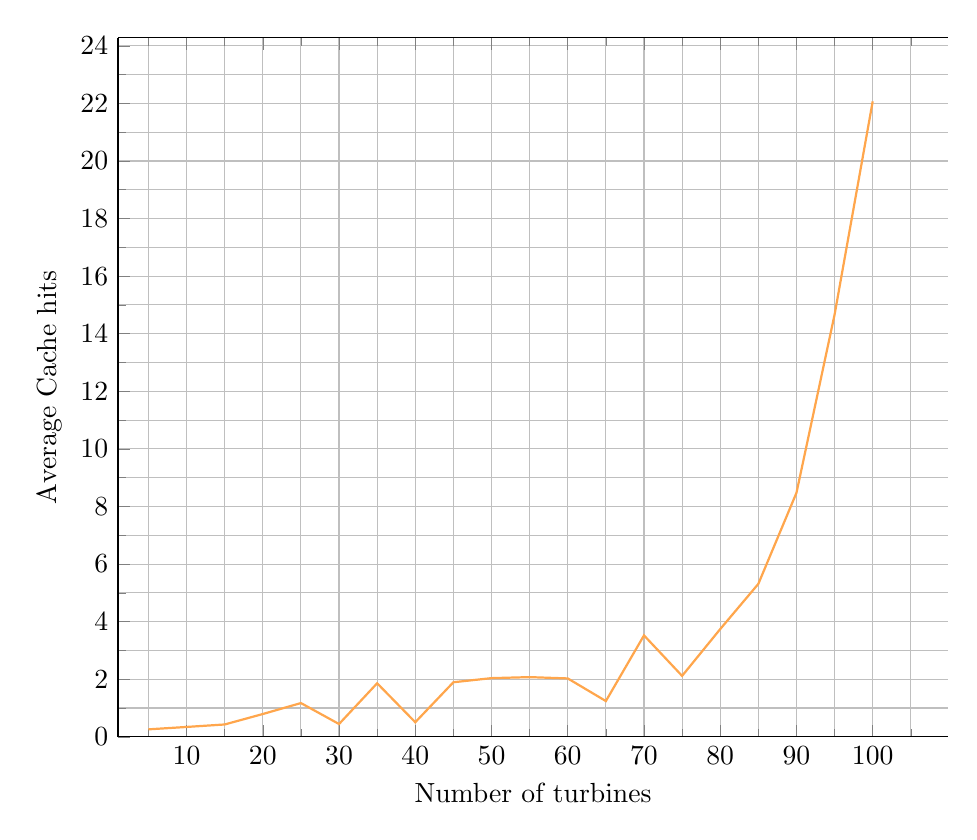
\begin{tikzpicture}
\begin{axis}
[
width=\resultsFigureWidthScale\textwidth,
axis y line*=left,
xlabel=Number of turbines,
ymin = 0,
xmin = 1,
ylabel=Average Cache hits,
%xtick={1, 2, 3, 4, 5, 6, 7, 8, 9, 10, 11, 12, 13, 14, 15, 16, 17, 18, 19, 20},
%xticklabels={5, 10, 15, 20, 25, 30, 35, 40, 45, 50, 55, 60, 65, 70, 75, 80, 85, 90, 95, 100},
%boxplot/draw direction=y,
grid=both,
minor tick num=1
]
%\buildBoxPlot[black]{0}{0}{0}{0}{0}
%\buildBoxPlot[black]{0}{0}{0}{0}{0}
%\buildBoxPlot[black]{0}{0}{0}{0}{0}
%\buildBoxPlot[black]{0}{0}{0}{0}{0}
%\buildBoxPlot[black]{0}{0}{0}{0}{0}
%\buildBoxPlot[black]{0}{0}{0}{0}{0}
%\buildBoxPlot[black]{0}{0}{0}{0}{0}
%\buildBoxPlot[black]{0}{0}{0}{0}{0}
%\buildBoxPlot[black]{0}{0}{0}{0}{0}
%\buildBoxPlot[black]{0}{0}{0}{0}{0}
%\buildBoxPlot[black]{0}{0}{0}{0}{0}
%\buildBoxPlot[black]{0}{0}{0}{0}{0}
%\buildBoxPlot[black]{0}{0}{0}{0}{0}
%\buildBoxPlot[black]{0}{0}{0}{0}{0}
%\buildBoxPlot[black]{0}{0}{0}{0}{0}
%\buildBoxPlot[black]{0}{0}{0}{0}{0}
%\buildBoxPlot[black]{0}{0}{0}{0}{0}
%\buildBoxPlot[black]{0}{0}{0}{0}{0}
%\buildBoxPlot[black]{0}{0}{0}{0}{0}
%\buildBoxPlot[black]{0}{0}{0}{0}{0}
\addplot[thick, orange!70] coordinates {
	(5 ,0.2591015249347438)
	(10 ,0.3423283799799435)
	(15 ,0.4286200856364344)
	(20 ,0.7913519050319182)
	(25 ,1.171919068056407)
	(30 ,0.4440826120490188)
	(35 ,1.8595523144717856)
	(40 ,0.506366007056297)
	(45 ,1.8951768000539848)
	(50 ,2.037951753081981)
	(55 ,2.0728170589196186)
	(60 ,2.0275369832294468)
	(65 ,1.2416290071090674)
	(70 ,3.5220372523313626)
	(75 ,2.115832267020478)
	(80 ,3.7417427229878832)
	(85 ,5.311682134712245)
	(90 ,8.473847137142263)
	(95 ,14.663734246038112)
	(100 ,22.06932793366117)
};
\end{axis}
\end{tikzpicture}
	\caption{Decentralized solution variable number of turbines experiment 1}
	\label{fig:exp:decen:turbines_cache}
\end{figure}


\cref{fig:exp:decen:turbines_cache} show the amount of cache reads the simulation had during part 2 of the experiment.
The plot almost lines up with a exponential curve. Also \cref{fig:exp:decen:turbines,fig:exp:decen:turbines_cache} seams to suddenly increase around 65 ms.

\subsection{Discussion}
\label{sec:disc:turbinesVScycletime}
This section address the \ref{PS:Q:Performance} problem of \cref{sec:problemStatement}.

In the current Siemens system the regulation cycle time of a single Park Pilot scales linearly with the number of turbines.
The aim of the decentralized solution is to detach the regulation cycle time from the number of turbines. 
Looking at \cref{fig:exp:decen:turbines} we see that the decentralized solution seems to be independent of the number of turbines if the number of turbines is sufficiently low.
From 5 to 65 turbines the regulation cycle time is nearly constant at 20 ms.
The near constant regulation cycle time is caused by the fact that the regulation cycle in the decentralized solution is not forced to wait for data before running the regulation algorithm because data is continually shared between turbines. Adding a turbine to the decentralized solution adds an extra turbine state to factor into the setpoint calculation in the regulation algorithm. This and the added network traffic for the new turbine is the consequence of adding new turbines.

When looking at regulation cycle time of the decentralized solution we must also look at the number of cache reads.
As explained in \cref{sec:exp:performance} a cache read happens when a turbine does not provide a new turbine state package before the next regulation cycle is started.
This forces the regulation cycle to use old data read from cache.
Looking at \cref{fig:exp:decen:turbines_cache} we see that the average number of cache reads in the decentralized solution are below 2 and increasing slightly until we reach 65 turbines. From there the number of cache reads increase exponentially.

The increase in regulation cycle time and cache reads when the number of turbines reaches 65 can be explained by the fact that the network equipment of the test setup is approaching maximum throughput capacity which may cause lost or delayed network packages.
Since regulation cycle time in the decentralized system is dependent on the reception time of the oldest turbine state package as explained in \cref{sec:exp:performance} the loss or delay of network packages has a direct impact on regulation cycle time.
Similarly lost or delayed network packages increases the use of cached data. The increased regulation cycle time and cache reads are thus not a limitation of the decentralized solution but a limitation imposed by the test setup. In order to create a realistic comparison we must disregard the results that are a direct effect of the limitations of our test setup.

Disregarding the limitations imposed by the test setup we see that the regulation cycle time is constant. In terms of regulation cycle time the decentralized solution scales indefinitely. As stated above there is a small increase in regulation cycle time for every turbine added because the state of this turbine has to be taken into consideration when calculating new setpoints on all other turbines. This time addition is not visible on \cref{fig:exp:decen:turbines}. Thus the regulation cycle time will be affected by the addition of turbines but the effect is so small that it is indistinguishable by other factors. Looking at the raw test data 

Still disregarding the limitations imposed by the test setup when looking at the scale factor of the number of cache reads we see another result. The number of cache reads increases slowly with a factor of around 1 cache read for every 30 turbines added, which gives a scale factor of $1 / 30 = 0.033$.

The number of cache reads can be reduced by increasing the regulation cycle time as presented in \cref{fig:exp:decen:sleep-cache}.
Thus the factor deciding the time of the regulation cycle is the maximum number of average cache reads accepted for a single regulation cycle.
